\section*{第七章 空间向量及其应用}

\section*{一、空间向量及其运算、空间向量基本定理}

\section*{【典型题型和解题技巧】}

本专题的学习,需要在平面向量的基础上,利用类比的方法理解空间向量的概念和运算, 体会平面向量和空间向量的共性和差异. 一方面要学会把空间中共面向量的问题化归为平面向量问题处理, 另一方面要学会把对平面向量所建立的理论进行类比与提升, 建立空间向量基本定理.

例 1 如图 1,已知平行六面体 ${ABCD} - {A}_{1}{B}_{1}{C}_{1}{D}_{1}$ 中,

(1)与 $\vv{AB}$ 相等的向量有\blkda{}；

(2) $\vv{A{A}_{1}}$ 的负向量有\blkda{};

( 3 )与 $\vv{AC}$ 平行的向量有\blkda{}.

分析 空间中, 向量的模、零向量、单位向量、相等向量、负向量、平行向量、两个非零向量的夹角等概念与平面向量相应的概念一致.

\begin{center}
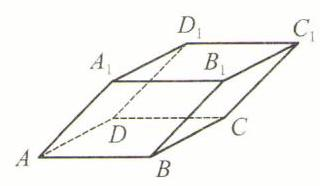
\includegraphics[width=0.2\textwidth]{bodyxb/src/bo_d20aucref24c73anc48g_222_1169_1118_320_186_0.jpg}
\end{center}


(图 1)

解 (1) $\vv{DC},\vv{{D}_{1}{C}_{1}},\vv{{A}_{1}{B}_{1}}$ . (2) $\vv{{A}_{1}A},\vv{{B}_{1}B},\vv{{C}_{1}C},\vv{{D}_{1}D}$ .

(3) $\vv{CA},\vv{{A}_{1}{C}_{1}},\vv{{C}_{1}{A}_{1}}$ .

例 2 已知正方体 ${ABCD} - {A}^{\prime }{B}^{\prime }{C}^{\prime }{D}^{\prime }$ 的中心为点 $O$ ,有以下四个命题:

① $\vv{AO} = \vv{O{C}^{\prime }}$ ；

② $\vv{OA} - \vv{O{A}^{\prime }} = \vv{OC} - \vv{O{C}^{\prime }}$ ；

③ $\vv{OA} + \vv{O{B}^{\prime }} + \vv{O{C}^{\prime }} + \vv{OD} = \vv{0}$ ；

④ $\vv{OA} + \vv{OB} + \vv{OC} + \vv{OD} = \vv{O{A}^{\prime }} + \vv{O{B}^{\prime }} + \vv{O{C}^{\prime }} + \vv{O{D}^{\prime }}$ ；

其中正确的命题是\blkda{}(填序号).

解 如图 2,①中, $O$ 是线段 $A{C}^{\prime }$ 的中点,故向量 $\vv{AO} = \vv{O{C}^{\prime }}$ ,①正确;

②中, $\vv{OA} - \vv{O{A}^{\prime }} = \vv{{A}^{\prime }A}$ , $\vv{OC} - \vv{O{C}^{\prime }} = \vv{{C}^{\prime }C}$ ,由于 $\vv{{A}^{\prime }A} = \vv{{C}^{\prime }C}$ ,故②正确；

\begin{center}
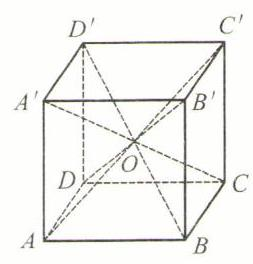
\includegraphics[width=0.2\textwidth]{bodyxb/src/bo_d20aucref24c73anc48g_222_1236_1807_253_264_0.jpg}
\end{center}


(图 2)

③中,因为 $\vv{OA} =  - \vv{O{C}^{\prime }},\vv{OD} =  - \vv{O{B}^{\prime }}$ ,所以 $\vv{OA} + \vv{O{B}^{\prime }} + \vv{O{C}^{\prime }} + \vv{OD} = \vv{0}$ , 故③正确;

④中,同③理,可知 $\vv{OA} + \vv{OB} + \vv{OC} + \vv{OD} + \vv{O{A}^{\prime }} + \vv{O{B}^{\prime }} + \vv{O{C}^{\prime }} + \vv{O{D}^{\prime }} =$ 0,记正方形 ${ABCD}$ 的中心为点 $E$ ,则 $\vv{OA} + \vv{OB} + \vv{OC} + \vv{OD} = 4\vv{OE} \neq  \vv{0}$ ,所以 ④不正确.

所以正确的是①②③.

例 3 在三棱锥 $O - {ABC}$ 中, $D$ 为 ${BC}$ 中点, $E$ 为 ${AD}$ 中点,设 $\vv{OA} = \vv{a},\vv{OB} = \vv{b},\vv{OC} = \vv{c}$ ,用 $a,b,c$ 表示向量 $\vv{OE} =$ \blkda{}.

解 如图 3 , 利用空间向量的线性运算, 可得

\begin{center}
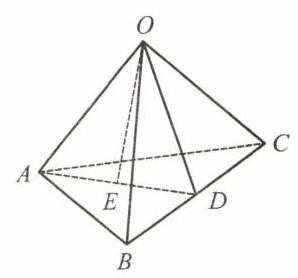
\includegraphics[width=0.2\textwidth]{bodyxb/src/bo_d20aucref24c73anc48g_223_1118_308_298_278_0.jpg}
\end{center}


(图 3)

$\vv{OE} = \dfrac{1}{2}\left( {\vv{OA} + \vv{OD}}\right)  = \dfrac{1}{2}\vv{OA} + \dfrac{1}{4}\left( {\vv{OB} + \vv{OC}}\right)  = \dfrac{1}{2}\vv{a} + \dfrac{1}{4}\vv{b} + \dfrac{1}{4}\vv{c}.$

例 4 在四面体 ${ABCD}$ 中,已知 ${AB} \bot  {CD},{AC} \bot  {BD}$ .

求证: ${AD}\bot {BC}$ .

分析 本题除了可以运用三垂线定理进行证明, 还可以借助空间向量进行证明.

证明 记 $\vv{AB} = \vv{a},\vv{AC} = \vv{b},\vv{AD} = \vv{c}$ ,

由 ${AB} \bot  {CD}$ 得, $\vv{AB} \cdot  \vv{CD} = \vv{a} \cdot  \left( {\vv{c} - \vv{b}}\right)  = 0$ ,故 $\vv{a} \cdot  \vv{b} = \vv{a} \cdot  \vv{c}$ .

由 ${AC} \bot  {BD}$ 得, $\vv{AC} \cdot  \vv{BD} = \vv{b} \cdot  \left( {\vv{c} - \vv{a}}\right)  = 0$ ,故 $\vv{a} \cdot  \vv{b} = \vv{b} \cdot  \vv{c}$ .

所以 $\vv{a} \cdot  \vv{b} = \vv{b} \cdot  \vv{c} = \vv{c} \cdot  \vv{a}$ ,所以 $\vv{AD} \cdot  \vv{BC} = \vv{c} \cdot  \left( {\vv{b} - \vv{a}}\right)  = 0$ ,故 ${AD} \bot  {BC}$ .

例 5 在正四面体 ${ABCD}$ 中, $E,F$ 分别是棱 ${BC},{AD}$ 的中点,求 $\vv{AE},\vv{CF}$ 的夹角大小.

分析 可以以 $\vv{AB},\vv{AC},\vv{AD}$ 为基向量,分别表示出向量 $\vv{AE}$ 与 $\vv{CF}$ ,再利用向量的数量积, 求出 $\vv{AE},\vv{CF}$ 的夹角.

证明 不妨设正四面体 ${ABCD}$ 棱长为 1,记 $\vv{AB} = \vv{a},\vv{AC} = \vv{b},\vv{AD} = \vv{c}$ ,

则 $\left| \vv{a}\right|  = \left| \vv{b}\right|  = \left| \vv{c}\right|  = 1$ ,且 $\vv{a} \cdot  \vv{b} = \vv{b} \cdot  \vv{c} = \vv{c} \cdot  \vv{a} = \dfrac{1}{2}$ .

因为 $\vv{AE} = \dfrac{1}{2}\left( {\vv{a} + \vv{b}}\right) ,\vv{CF} = \vv{CA} + \vv{AF} =  - \vv{b} + \dfrac{1}{2}\vv{c}$ ,

所以 $\vv{AE} \cdot  \vv{CF} = \dfrac{1}{2}\left( {\vv{a} + \vv{b}}\right)  \cdot  \left( {-\vv{b} + \dfrac{1}{2}\vv{c}}\right)  =  - \dfrac{1}{2}\vv{a} \cdot  \vv{b} + \dfrac{1}{4}\vv{a} \cdot  \vv{c} - \dfrac{1}{2}{\vv{b}}^{2} + \dfrac{1}{4}\vv{b} \cdot  \vv{c} =  - \dfrac{1}{2}$ .

又 $\left| \vv{AE}\right|  = \dfrac{1}{2}\sqrt{{\left( \vv{a} + \vv{b}\right) }^{2}} = \dfrac{1}{2}\sqrt{{\vv{a}}^{2} + 2\vv{a} \cdot  \vv{b} + {\vv{b}}^{2}} = \dfrac{\sqrt{3}}{2},\left| \vv{CF}\right|  = \sqrt{{\left( -\vv{b} + \dfrac{1}{2}\vv{c}\right) }^{2}} = \dfrac{\sqrt{3}}{2}$ ,

所以 $\cos \langle \vv{AE},\vv{CF}\rangle  = \dfrac{\vv{AE} \cdot  \vv{CF}}{\left| \vv{AE}\right| \left| \vv{CF}\right| } = \dfrac{-\dfrac{1}{2}}{\dfrac{\sqrt{3}}{2} \cdot  \dfrac{\sqrt{3}}{2}} =  - \dfrac{2}{3}$ ,所以 $\vv{AE},\vv{CF}$ 的夹角大小为 $\pi  -$ arccos $\dfrac{2}{3}$ .

例 6 如图 4,在四棱台 ${ABCD} - {A}^{\prime }{B}^{\prime }{C}^{\prime }{D}^{\prime }$ 中, $A{A}^{\prime } = 4,\angle {BAD} =$  $\angle {BA}{A}^{\prime } = \angle {DA}{A}^{\prime } = {60}^{ \circ  }$ ,则 $\left| {\vv{D{B}^{\prime }} - \left( {x\vv{AB} + y\vv{AD}}\right) }\right| \left( {x,y \in  \mathbf{R}}\right)$ 的最小值为\blkda{}.

\begin{center}
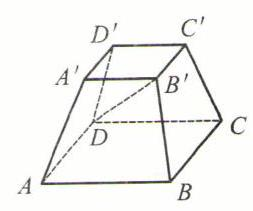
\includegraphics[width=0.2\textwidth]{bodyxb/src/bo_d20aucref24c73anc48g_223_1175_1832_253_211_0.jpg}
\end{center}


(图 4)

分析 可作向量 $\vv{DM} = x\vv{AB} + y\vv{AD}$ ,则点 $M$ 在平面 ${ABCD}$ 上,

且 $\left| {\vv{D{B}^{\prime }} - \left( {x\vv{AB} + y\vv{AD}}\right) }\right|  = \left| {\vv{D{B}^{\prime }} - \vv{DM}}\right|  = \left| \vv{M{B}^{\prime }}\right|$ ,故当 $M{B}^{\prime } \bot$ 平面 ${ABCD}$ 时, $\left| {\vv{D{B}^{\prime }} - \left( {x\vv{AB} + y\vv{AD}}\right) }\right|$ 最小,问题转化为求该四棱台的高.

解 由分析知, $\left| {\vv{D{B}^{\prime }} - \left( {x\vv{AB} + y\vv{AD}}\right) }\right|$ 的最小值为四棱台 ${ABCD} - {A}^{\prime }{B}^{\prime }{C}^{\prime }{D}^{\prime }$ 的高,设 $A{A}^{\prime }$ 与平面 ${ABCD}$ 所成角为 $\theta$ ,则 $\cos \theta  \cdot  \cos {30}^{ \circ  } = \cos {60}^{ \circ  }$ ,故 $\cos \theta  = \dfrac{\sqrt{3}}{3}$ ,该四棱台的高为 $\left| {A{A}^{\prime }}\right| \sin \theta$  $= 4 \times  \sqrt{1 - \dfrac{1}{3}} = \dfrac{4}{3}\sqrt{6}$ ,所以 $\left| {\vv{D{B}^{\prime }} - \left( {x\vv{AB} + y\vv{AD}}\right) }\right|$ 的最小值为 $\dfrac{4}{3}\sqrt{6}$ .

例 7 已知 $a,b,c$ 是空间中不共面的向量,且 $\vv{AB} = {2a} - b + c,\vv{AC} = a + {2b} - c,\vv{AD} =  - a$  $+ {xb} + {yc}$ .

(1)若 $B,C,D$ 三点共线,求 $x$ , $y$ 的值；

(2)若 $A,B,C,D$ 四点共面,求 ${xy}$ 的最大值.

分析 (1)若 $B,C,D$ 三点共线,由向量共线定理,可设 $\vv{BD} = \lambda \vv{BC}$ ,列方程求 $x$ , $y$ 的值；

(2)若 $A,B,C,D$ 四点共面,由向量共面定理,可设 $\vv{AD} = \lambda \vv{AB} + \mu \vv{AC}$ ,从而求得 $x,y$ 之间的关系式,进一步可求 ${xy}$ 的最大值.

解 (1) $\vv{BD} = \vv{AD} - \vv{AB} =  - 3\vv{a} + \left( {x + 1}\right) \vv{b} + \left( {y - 1}\right) \vv{c},\vv{BC} = \vv{AC} - \vv{AB} =  - \vv{a} + 3\vv{b} - 2\vv{c}$ ,由向量共线定理知,存在 $\lambda  \in  \mathbf{R}$ 使得 $\vv{BD} = \lambda \vv{BC}$ ,故 $\left\{  \begin{array}{l}  - 3 =  - \lambda , \\  x + 1 = {3\lambda }, \\  y - 1 =  - {2\lambda }, \end{array}\right.$ 解得 $\left\{  \begin{array}{l} x = 8, \\  y =  - 5. \end{array}\right.$

(2)显然 $\vv{AB},\vv{AC}$ 不共线,由向量共面定理知,存在唯一的 $\left( {\lambda ,\mu }\right)$ 使得 $\vv{AD} = \lambda \vv{AB} + \mu \vv{AC}$ ,

即 $- \vv{a} + x\vv{b} + {yc} = \lambda \left( {2\vv{a} - \vv{b} + \vv{c}}\right)  + \mu \left( {\vv{a} + 2\vv{b} - \vv{c}}\right)$ ,故 $\left\{  \begin{array}{l}  - 1 = {2\lambda } + \mu , \\  x =  - \lambda  + {2\mu }, \\  y = \lambda  - \mu , \end{array}\right.$ 整理得 ${3x} + {5y} =  - 1$ ,所以

${xy} = x \cdot  \dfrac{-1 - {3x}}{5} =  - \dfrac{3}{5}{\left( x + \dfrac{1}{6}\right) }^{2} + \dfrac{1}{60} \leq  \dfrac{1}{60}$ ,当且仅当 $\left\{  \begin{array}{l} x =  - \dfrac{1}{6}, \\  y =  - \dfrac{1}{10} \end{array}\right.$ 时等号成立,所以 ${xy}$ 的最大值为 $\dfrac{1}{60}$ .

\section*{【训练题】}

\section*{(A)}

1. 对于空间任意两个非零向量 $a,b,$ “ $a//b$ ”是“ $\langle a,b\rangle  = 0$ ”的(   )

(A) 充分不必要条件. (B) 必要不充分条件.

(C) 充要条件. (D) 既不充分也不必要条件.

2. 在四面体 ${ABCD}$ 中, $E$ 为棱 ${BC}$ 的中点,则 $\vv{DA} - \dfrac{1}{2}\left( {\vv{DB} + \vv{DC}}\right)  =$ (   )

(A) $- \vv{AE}$ . (B) $- \vv{AB}$ .

(C) $\vv{\Lambda E}$ . (D) $\vv{AB}$ .

3. 在四棱锥 $P - {ABCD}$ 中,底面 ${ABCD}$ 是正方形, $E$ 是 ${PD}$ 的中点,若 $\vv{PA} = \vv{a},\vv{PB} = \vv{b}$ ,

$\vv{PC} = c$ ,则 $\vv{BE} =$ (   )

(A) $\dfrac{1}{2}\vv{a} - \dfrac{1}{2}\vv{b} + \dfrac{1}{2}\vv{c}$ . (B) $\dfrac{1}{2}\vv{a} - \dfrac{3}{2}\vv{b} - \dfrac{1}{2}\vv{c}$ .

(C) $\dfrac{1}{2}\vv{a} - \dfrac{3}{2}\vv{b} + \dfrac{1}{2}\vv{c}$ . (D) $\dfrac{1}{2}\vv{a} - \dfrac{1}{2}\vv{b} + \dfrac{3}{2}\vv{c}$ .

4. 已知空间不共线的向量 $\vv{a},\vv{b}$ ,且 $\vv{AB} = \vv{a} + 2\vv{b},\vv{BC} =  - 5\vv{a} + 6\vv{b},\vv{CD} = 7\vv{a} - 2\vv{b}$ ,则一定共线的三点是(   )

(A) $A,B,C$ . (B) $B,C,D$ . (C) $A,B,D$ . (D) $A,C,D$ .

5. 设 $O$ 是 $\bigtriangleup {ABC}$ 所在平面外的一点, $\vv{OA} \cdot  \vv{OC} = \vv{OB} \cdot  \vv{OC}$ ,则直线 ${AB}$ 与直线 ${OC}$ 的位置关系是(   )

(A) 平行. (B) 垂直. (C) 重合. (D) 相交但不垂直.

6. 如图,已知四面体 ${ABCD}$ 的棱长都是 2, $M$ 为棱 ${AD}$ 的中点,则 $\vv{AB} \cdot  \vv{CM}$ 的值为(   )

(A) 1 . (B) -1 . (C) -2 . (D) 2 .

\begin{center}
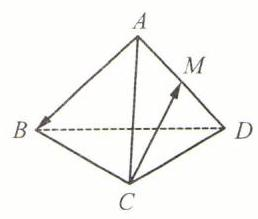
\includegraphics[width=0.2\textwidth]{bodyxb/src/bo_d20aucref24c73anc48g_225_242_901_258_219_0.jpg}
\end{center}


(第 6 题)

\begin{center}
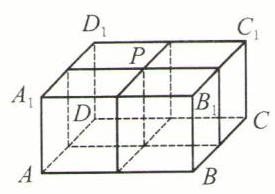
\includegraphics[width=0.2\textwidth]{bodyxb/src/bo_d20aucref24c73anc48g_225_617_923_275_194_0.jpg}
\end{center}


(第 7 题)

\begin{center}
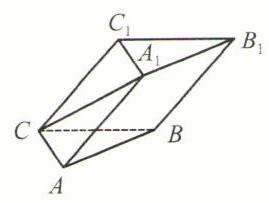
\includegraphics[width=0.2\textwidth]{bodyxb/src/bo_d20aucref24c73anc48g_225_1005_912_269_203_0.jpg}
\end{center}


(第 8 题)

7. 如图,由四个棱长为 1 的正方体组合成的正四棱柱 ${ABCD} - {A}_{1}{B}_{1}{C}_{1}{D}_{1},P$ 是正方形 ${A}_{1}{B}_{1}{C}_{1}{D}_{1}$ 的中心,则向量 $\vv{A{A}_{1}} \cdot  \vv{AP} =$ (   )

(A) 1 . (B) 2. (C) 4 . (D) 8.

8. 如图,在斜三棱柱 ${ABC} - {A}_{1}{B}_{1}{C}_{1}$ 中, ${AC} = {BC} = {C{C}_{1}} = 4,\angle {{BC}{C}_{1}} = \angle {{AC}{C}_{1}} = \dfrac{\pi }{3},\angle {ACB}$  $= \dfrac{\pi }{4}$ ,则 $\vv{C{A}_{1}} \cdot  \left( {\vv{CB} + \vv{CA}}\right)  =$ (   )

(A) 48. (B) 32. (C) ${32} + 8\sqrt{2}$ . (D) ${32} - 8\sqrt{2}$ .

9. 已知空间向量 $a,b,c$ 两两夹角为 ${60}^{ \circ  }$ ,且 $\left| a\right|  = \left| b\right|  = \left| c\right|  = 1$ ,则 $\left| {a - b + {2c}}\right|  =$ \blkda{}.

10. 已知 $\vv{a},\vv{b}$ 是两个空间向量,若 $\left| \vv{a}\right|  = 2,\left| \vv{b}\right|  = 2,\left| {\vv{a} - \vv{b}}\right|  = \sqrt{7}$ ,则 $\cos \langle \vv{a},\vv{b}\rangle  =$ \blkda{}.

11. 如图,在四面体 ${PABC}$ 中, $E$ 是 ${AC}$ 的中点, $\vv{BF} = 3\vv{FP}$ ,设 $\vv{PA} = a$ , $\vv{PB} = \vv{b},\vv{PC} = \vv{c}$ ,则 $\vv{FE} =$ \blkda{}.(用 $\vv{a},\vv{b},\vv{c}$ 表示)

\begin{center}
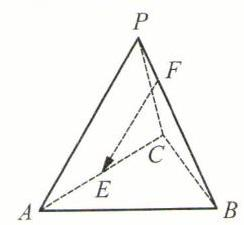
\includegraphics[width=0.2\textwidth]{bodyxb/src/bo_d20aucref24c73anc48g_225_1199_1737_244_225_0.jpg}
\end{center}


(第 11 题)

12. 已知 ${OABC}$ 是空间四面体,空间的一点 $M$ 满足 $\vv{OM} = \dfrac{1}{2}\vv{OA} + \dfrac{1}{3}\vv{OB} +$  $\lambda \vv{OC}$ . 若 $\vv{MA},\vv{MB},\vv{MC}$ 共面,则 $\lambda  =$ \blkda{}.

13. 已知空间向量 $\vv{PA},\vv{PB},\vv{PC}$ 的模长分别为1,2,3,且两两夹角均为 $\dfrac{\pi }{3},G$ 为 $\bigtriangleup  {ABC}$ 的重心,则 $\left| \vv{PG}\right|  =$ \blkda{}.

14. 如图,四面体 ${OABC}$ 中, $\angle {OAB} = \angle {OAC} = \angle {BAC} = {60}^{ \circ  },{OA} = 1,{AB}$  $= 1,{AC} = 3,D,E$ 分别是 ${OA},{BC}$ 的中点,则 ${DE} =$ \blkda{}.

\begin{center}
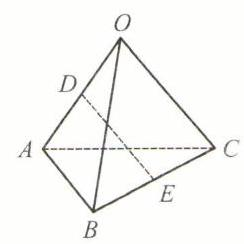
\includegraphics[width=0.2\textwidth]{bodyxb/src/bo_d20aucref24c73anc48g_226_1241_121_244_244_0.jpg}
\end{center}


(第 14 题)

15. 如图,在长方体 ${ABCD} - {A}_{1}{B}_{1}{C}_{1}{D}_{1}$ 中, ${AB} = 3,{AD} = 2,{AA}_{1} = 1$ ,以长方体的八个顶点中的两点为起点和终点的向量中, (1)单位向量共有多少个？ (2)试写出与 $\vv{AB}$ 相等的所有向量； (3) 试写出 $\vv{A{A}_{1}}$ 的相反向量. 16. 如图,已知矩形 ${ABCD},P$ 为平面 ${ABCD}$ 外一点,且 ${PA} \bot$ 平面 ${ABCD},M,N$ 分别为 ${PC}$ , ${PD}$ 上的点,且 ${PM} : {MC} = 2 : 1,{PN} = {ND}$ ,求满足 $\vv{MN} = x\vv{AB} + y\vv{AD} + z\vv{AP}$ 的实数 $x$ , $y,z$ 的值.

\begin{center}
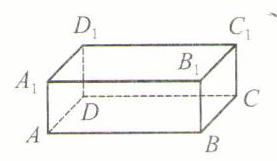
\includegraphics[width=0.2\textwidth]{bodyxb/src/bo_d20aucref24c73anc48g_226_283_794_277_161_0.jpg}
\end{center}


(第 15 题)

\begin{center}
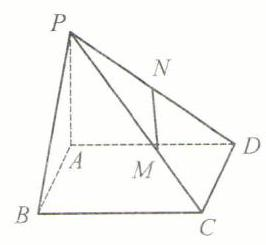
\includegraphics[width=0.2\textwidth]{bodyxb/src/bo_d20aucref24c73anc48g_226_662_708_266_245_0.jpg}
\end{center}


(第 16 题)

\begin{center}
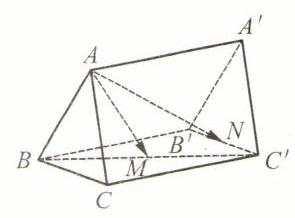
\includegraphics[width=0.2\textwidth]{bodyxb/src/bo_d20aucref24c73anc48g_226_1040_733_295_218_0.jpg}
\end{center}


(第 17 题)

17. 如图,在三棱柱 ${ABC} - {A}^{\prime }{B}^{\prime }{C}^{\prime }$ 中,已知 $\vv{A{A}^{\prime }} = a,\vv{AB} = b,\vv{AC} = c,M,N$ 分别是 $B{C}^{\prime },{B}^{\prime }{C}^{\prime }$ 的中点,试用一组基 $\{ \vv{a},\vv{b},\vv{c}\}$ 表示向量 $\vv{AM},\vv{AN}$ .

18. 已知向量 $a,b,c$ 不共面, $\vv{AB} = {4a} + {5b} + {3c},\vv{AC} = {2a} + {3b} + c,\vv{AD} = {6a} + {7b} + {5c}$ . 求证: $B$ , $C,D$ 三点共线.

19. 如图,正四面体 ${ABCD}$ 的棱长为 $1,E,F$ 分别为棱 ${BC},{CD}$ 的中点, $G$ 为线段 ${AF}$ 的中点.

(1)用 $\vv{AB},\vv{AC},\vv{AD}$ 表示 $\vv{EG}$ ；

(2) 求 $\vv{EG} \cdot  \vv{AB}$ 的值.

\begin{center}
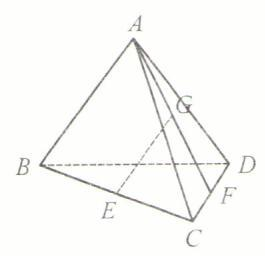
\includegraphics[width=0.2\textwidth]{bodyxb/src/bo_d20aucref24c73anc48g_226_480_1440_265_256_0.jpg}
\end{center}


(第 19 题)

\begin{center}
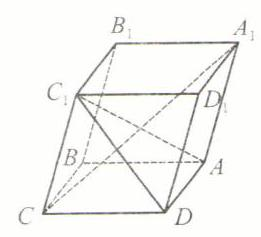
\includegraphics[width=0.2\textwidth]{bodyxb/src/bo_d20aucref24c73anc48g_226_884_1458_261_237_0.jpg}
\end{center}


(第 20 题)

20. 如图,平行六面体 ${ABCD} - {A}_{1}{B}_{1}{C}_{1}{D}_{1}$ 的底面是菱形,且 $\angle {C}_{1}{CB} = \angle {C}_{1}{CD} = \angle {BCD} =$  ${60}^{ \circ  },{CD} = 1,C{C}_{1} = 2$ .

(1) 求 ${A}_{1}C$ 的长;

(2)求异面直线 $C{A}_{1}$ 与 $D{C}_{1}$ 所成的角的余弦值.

21. 对于空间向量,给出下列命题,其中正确的是(   )

(A)若 $a \cdot  b < 0$ ,则 $\langle a,b\rangle$ 是钝角.

(B)若 $\vv{AB} + \vv{CD} = \vv{0}$ ,则 $\vv{AB}$ 与 $\vv{CD}$ 一定共线.

(C) 若 $\vv{AB} = \vv{CD}$ ,则 ${AB}$ 与 ${CD}$ 为同一线段.

(D) 非零向量 $a,b,c$ 满足 $a$ 与 $b,b$ 与 $c,c$ 与 $a$ 都是共面向量,则 $a,b,c$ 必共面.

22. 下列选项中, 不正确的命题是 (   )

(A) 若两条不同直线 $l,m$ 的方向向量为 ${\vv{v}}_{1},{\vv{v}}_{2}$ ,则 $l//m \Leftrightarrow  {\vv{v}}_{1}//{\vv{v}}_{2}$ .

(B) 若 $\{ \vv{OA},\vv{OB},\vv{OC}\}$ 是空间向量的一组基底,且 $\vv{OD} = \dfrac{1}{3}\vv{OA} + \dfrac{1}{3}\vv{OB} + \dfrac{1}{3}\vv{OC}$ ,则点 $D$ 在平面 ${ABC}$ 内,且 $D$ 为 $\bigtriangleup {ABC}$ 的重心.

(C) 若 $\{ a,b,c\}$ 是空间向量的一组基底,则 $\{ a + b,{2c},a + b + c\}$ 也是空间向量的一组基底.

(D) 若空间向量 $a,b,c$ 共面,则存在不全为 0 的实数 $x,y,z$ 使 ${xa} + {yb} + {zc} = 0$ .

23. 对于空间任一点 $O$ 和不共线的三点 $A,B,C$ ,有 $\vv{OP} = x\vv{OA} + y\vv{OB} + z\vv{OC}$ ,则 $x + y + z = 1$ 是 $P,A,B,C$ 四点共面的 (   )

(A) 必要不充分条件. (B) 充分不必要条件.

(C) 充要条件. (D) 既不充分又不必要条件.

24. 已知棱长为 1 的正方体 ${ABCD} - {A}_{1}{B}_{1}{C}_{1}{D}_{1}$ ,以正方体中心为球心的球 $O$ 与正方体的各条棱相切,若 $P$ 为球面上的动点,则 $\vv{PA} \cdot  \vv{PB}$ 的最大值为 (   )

(A) 2 . (B) $\dfrac{7}{4}$ . (C) $\dfrac{3}{4}$ . (D) $\dfrac{1}{4}$ .

25. 空间中,同起点的两个向量 $a,b$ ,满足 $a \cdot  b = 2,\left| b\right|  = 1$ ,且存在实数 $t$ ,使得 $\left| a\right|  -$  $2\left| {\vv{a} + t\vv{b}}\right|  \geq  0$ 成立,则向量 $\vv{b}$ 确定时,由 $\vv{a}$ 构成的空间几何体的侧面积是 (   ).

(A) $\dfrac{4\pi }{3}$ . (B) $\dfrac{4\pi }{9}$ . (C) $\dfrac{8\pi }{3}$ . (D) $\dfrac{8\pi }{9}$ .

26. 已知三棱锥 $P - {ABC}$ ,点 $G$ 满足: $\vv{GP} + \vv{GA} + \vv{GB} + \vv{GC} = \vv{0}$ ,过点 $G$ 作平面,与直线 ${PA}$ , ${PB},{PC}$ 分别相交于 $D,E,F$ 三点,且 $\vv{PD} = x\vv{PA},\vv{PE} = y\vv{PB},\vv{PF} = z\vv{PC}$ ,则 $\dfrac{1}{x} + \dfrac{1}{y} + \dfrac{1}{z} =$ \blkda{}.

27. 如图所示,二面角 $\alpha  - l - \beta$ 的大小为 ${60}^{ \circ  },A,B$ 是棱 $l$ 上的两点, ${AC},{BD}$ 分别在半平面 $\alpha ,\beta$ 内,且 ${AC}\bot l,{BD}\bot l,{AB} = 4,{AC} = 6,{BD} = 8$ ,则 ${CD}$ 的长为\blkda{}.

\begin{center}
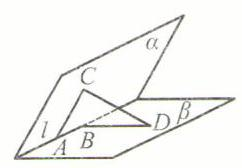
\includegraphics[width=0.2\textwidth]{bodyxb/src/bo_d20aucref24c73anc48g_227_283_1816_242_168_0.jpg}
\end{center}


(第 27 题)

\begin{center}
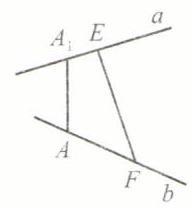
\includegraphics[width=0.2\textwidth]{bodyxb/src/bo_d20aucref24c73anc48g_227_636_1771_194_210_0.jpg}
\end{center}


(第 28 题)

\begin{center}
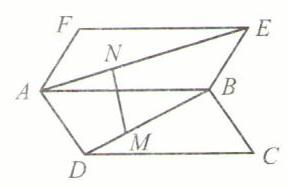
\includegraphics[width=0.2\textwidth]{bodyxb/src/bo_d20aucref24c73anc48g_227_941_1793_287_188_0.jpg}
\end{center}


(第 29 题)

28. 如图,两条异面直线 $a$ , $b$ 所成的角为 ${60}^{ \circ  }$ ,在直线 $a$ , $b$ 上分别取点 ${A}_{1}$ , $E$ 和点 $A$ , $F$ ,使 ${A}_{1}A$  $\bot  a,{A}_{1}A \bot  b$ . 已知 ${A}_{1}E = 1,{AF} = 2,{EF} = 3$ ,则 $\left| {A{A}_{1}}\right|  =$ \blkda{}.

29. 如图,在矩形 ${ABCD}$ 和 ${ABEF}$ 中, ${AB} = 4,{AD} = {AF} = 3,\angle {DAF} = \dfrac{\pi }{3},\vv{DM} = \lambda \vv{DB},\vv{AN} =$  $\lambda \vv{AE},0 < \lambda  < 1$ ,记 $\vv{AB} = \vv{a},\vv{AD} = \vv{b},\vv{AF} = \vv{c}$ .

(1)当 $\lambda  = \dfrac{1}{2}$ 时,求 ${MN}$ 与 ${AE}$ 夹角的余弦值；

(2)是否存在 $\lambda$ ,使得 ${MN} \bot$ 平面 ${ABCD}$ ？若存在,求出 $\lambda$ 的值,若不存在,请说明理由.

30. 如图,在底面 ${ABCD}$ 为菱形的平行六面体 ${ABCD} - {A}_{1}{B}_{1}{C}_{1}{D}_{1}$ 中, $M$ , $N$ 分别在棱 $A{A}_{1},C{C}_{1}$ 上,且 ${A}_{1}M = \dfrac{1}{3}A{A}_{1},{CN} = \dfrac{1}{3}C{C}_{1}$ ,且 $\angle {A}_{1}{AD}$  $= \angle {A}_{1}{AB} = \angle {DAB} = {60}^{ \circ  }$ .

\begin{center}
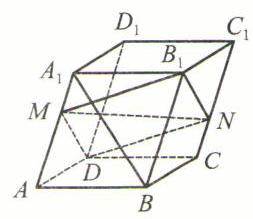
\includegraphics[width=0.2\textwidth]{bodyxb/src/bo_d20aucref24c73anc48g_228_1248_438_253_219_0.jpg}
\end{center}


(第 30 题)

(1)求证: $D,M,{B}_{1},N$ 共面；

(2)当 $\dfrac{A{A}_{1}}{AB}$ 为何值时, $A{C}_{1}\bot {A}_{1}B$ ；

(3)若 ${AB} = {A{A}_{1}} = 1$ ,且 $\vv{{A}_{1}P} = \dfrac{1}{2}\vv{{A}_{1}{C}_{1}}$ ,求 ${AP}$ 的长.

\section*{二、空间向量的坐标表示、空间向量在立体几何中的应用}

\section*{【典型题型和解题技巧】}

1. 空间向量的坐标表示.

建立空间直角坐标系 (右手系),把向量 $p$ 的起点放在坐标原点,该向量就直接用它的终点坐标(x, y, z)表示为 $p = \left( {x,y,z}\right)$ ,表示的意义: $p$ 是坐标轴正方向上的单位向量 $i,j$ 与 $k$ 的线性组合 $\mathbf{p} = x\vv{i} + y\vv{j} + z\mathbf{k}$ .

给定空间两点 $A\left( {{x}_{1},{y}_{1},{z}_{1}}\right)$ 与 $B\left( {{x}_{2},{y}_{2},{z}_{2}}\right)$ ,则 $\vv{AB} = \left( {{x}_{2} - {x}_{1},{y}_{2} - {y}_{1},{z}_{2} - {z}_{1}}\right)$ .

2. 坐标表示下的空间向量运算.

设 $\vv{a} = \left( {{x}_{1},{y}_{1},{z}_{1}}\right) ,\vv{b} = \left( {{x}_{2},{y}_{2},{z}_{2}}\right) ,\lambda  \in  \mathbf{R}$ ,则

(1) $\left| \vv{a}\right|  = \sqrt{{x}_{1}^{2} + {y}_{1}^{2} + {z}_{1}^{2}}$ ;

(2) $a \pm  b = \left( {{x}_{1} \pm  {x}_{2},{y}_{1} \pm  {y}_{2},{z}_{1} \pm  {z}_{2}}\right)$ ；

(3) $\lambda \vv{a} = \left( {\lambda {x}_{1},\lambda {y}_{1},\lambda {z}_{1}}\right)$ ；

(4) $\vv{a} \cdot  \vv{b} = {x}_{1}{x}_{2} + {y}_{1}{y}_{2} + {z}_{1}{z}_{2}$ .

3. 空间向量的夹角、平行与垂直.

设向量 $\vv{a} = \left( {{x}_{1},{y}_{1},{z}_{1}}\right) ,\vv{b} = \left( {{x}_{2},{y}_{2},{z}_{2}}\right)$ 均为非零向量,则

(1) $\cos \langle \vv{a},\vv{b}\rangle  = \dfrac{\vv{a} \cdot  \vv{b}}{\left| \vv{a}\right| \left| \vv{b}\right| } = \dfrac{{x}_{1}{x}_{2} + {y}_{1}{y}_{2} + {z}_{1}{z}_{2}}{\sqrt{{x}_{1}^{2} + {y}_{1}^{2} + {z}_{1}^{2}}\sqrt{{x}_{2}^{2} + {y}_{2}^{2} + {z}_{2}^{2}}}$ ;

(2) $a//b \Leftrightarrow$ 存在 $\lambda  \in  \mathbf{R}$ ,使得 $a = {\lambda b} \Leftrightarrow$ 存在 $\lambda  \in  \mathbf{R}$ ,使得 ${x}_{1} = \lambda {x}_{2},{y}_{1} = \lambda {y}_{2},{z}_{1} = \lambda {z}_{2}$ ；

(3) $\vv{a}\bot \vv{b} \Leftrightarrow  \vv{a} \cdot  \vv{b} = 0 \Leftrightarrow  {x}_{1}{x}_{2} + {y}_{1}{y}_{2} + {z}_{1}{z}_{2} = 0$ .

4. 空间向量在立体几何中的应用.

(1)判断空间直线与平面的平行与垂直.

设 ${\mathbf{r}}_{1},{\mathbf{r}}_{2}$ 分别是直线 $l,m$ 的方向向量, ${\vv{n}}_{1},{\vv{n}}_{2}$ 分别是平面 $\alpha ,\beta$ 的法向量.

① $l//m \Leftrightarrow  {\mathbf{r}}_{1}//{\mathbf{r}}_{2};l \bot  m \Leftrightarrow  {\mathbf{r}}_{1} \bot  {\mathbf{r}}_{2}$ ;

② $l \bot  \alpha  \Leftrightarrow  {\mathbf{r}}_{1}//{\vv{n}}_{1}$ ；直线 $l$ 在平面 $\alpha$ 外,则 $l//\alpha  \Leftrightarrow  {\mathbf{r}}_{1} \bot  {\vv{n}}_{1}$ ；

③ $\alpha //\beta  \Leftrightarrow  {\vv{n}}_{1}//{\vv{n}}_{2};\alpha  \bot  \beta  \Leftrightarrow  {\vv{n}}_{1} \bot  {\vv{n}}_{2}$ .

(2)求距离.

①平面外一点 $A$ 到平面的距离 $d = \dfrac{\left| \vv{n} \cdot  \vv{AB}\right| }{\left| \vv{n}\right| }$ ,其中 $\vv{n}$ 是平面的一个法向量, $B$ 是平面上任意一点;

②平面的平行线到平面的距离、平行平面的距离转化为点到平面的距离来处理.

(3) 求角.

设 ${\mathbf{r}}_{1},{\mathbf{r}}_{2}$ 分别是直线 $l,m$ 的方向向量, ${\vv{n}}_{1},{\vv{n}}_{2}$ 分别是平面 $\alpha ,\beta$ 的法向量.

① 直线 $l,m$ 的所成角 $\theta$ 的大小由公式 $\cos \theta  = \dfrac{\left| {\mathbf{r}}_{1} \cdot  {\mathbf{r}}_{2}\right| }{\left| {\mathbf{r}}_{1}\right| \left| {\mathbf{r}}_{2}\right| }$ 确定；

②直线 $l$ 与平面 $\alpha$ 的所成角 $\theta$ 的大小由公式 $\sin \theta  = \dfrac{\left| {\mathbf{r}}_{1} \cdot  {\vv{n}}_{1}\right| }{\left| {\mathbf{r}}_{1}\right| \left| {\vv{n}}_{1}\right| }$ 确定；

③平面 $\alpha ,\beta$ 所成的锐二面角 (或直二面角) $\theta$ 的大小由公式 $\cos \theta  = \dfrac{{n}_{1} \cdot  {n}_{2}}{\left| {n}_{1}\right| \left| {n}_{2}\right| }$ 确定.

例 1 已知 $A\left( {1, - 2, - 1}\right) ,B\left( {-1, - 4, - 5}\right) ,C\left( {5,1, - 3}\right)$ ,若 $\vv{AB} = 2\vv{CD}$ ,求 $\left| \vv{AB}\right|$ 及点 $D$ 的坐标.

分析 设点 $D$ 的坐标为(x, y, z),分别表示出 $\vv{AB},\vv{CD}$ 的坐标,根据向量的模的公式可求 $\left| \vv{AB}\right|$ ; 根据向量相等可以列出方程组,从而求出点 $D$ 的坐标.

解 设点 $D$ 的坐标为(x, y, z),则 $\vv{AB} = \left( {-2, - 2, - 4}\right) ,\vv{CD} = \left( {x - 5,y - 1,z + 3}\right)$ .

\[
\left| \vv{AB}\right|  = \sqrt{{\left( -2\right) }^{2} + {\left( -2\right) }^{2} + {\left( -4\right) }^{2}} = 2\sqrt{6}.
\]

因为 $\vv{AB} = 2\vv{CD}$ ,所以 $\left\{  \begin{array}{l} 2\left( {x - 5}\right)  =  - 2, \\  2\left( {y - 1}\right)  =  - 2, \\  2\left( {z + 3}\right)  =  - 4, \end{array}\right.$ 解得 $\left\{  \begin{array}{l} x = 4, \\  y = 0, \\  z =  - 5. \end{array}\right.$ 故点 $D$ 的坐标为(4,0, - 5).

例 2 已知 $\vv{a} = \left( {-2,3,2}\right) ,\vv{b} = \left( {1, - 5, - 1}\right) ,m \in  \mathbf{R}$ .

(1)若 ${ma} + b$ 与 ${2a} - {3b}$ 平行,求实数 $m$ 的值；

(2)若 ${ma} + b$ 与 ${2a} - {3b}$ 的夹角为钝角,求实数 $m$ 的取值范围.

分析 分别写出 ${ma} + b$ 与 ${2a} - {3b}$ 的坐标形式,(1) 可以利用两个向量平行的充要条件, 即存在 $\lambda  \in  \mathbf{R}$ 使 ${ma} + b = \lambda \left( {{2a} - {3b}}\right)$ ,从而求 $m$ 的值；(2)可以利用 $\left( {{ma} + b}\right)  \cdot  \left( {{2a} - {3b}}\right)  < 0$ 且 ${ma} + \vv{b}$ 与 $2\vv{a} - 3\vv{b}$ 不平行,从而求得 $m$ 的取值范围.

解 ${ma} + b = \left( {-{2m} + 1,{3m} - 5,{2m} - 1}\right) ,{2a} - {3b} = \left( {-7,{21},7}\right)$ .

(1)若 ${ma} + b$ 与 ${2a} - {3b}$ 平行,则存在 $\lambda  \in  \mathbf{R}$ 使 ${ma} + b = \lambda \left( {{2a} - {3b}}\right)$ ,故 $\left\{  \begin{array}{l}  - {2m} + 1 =  - {7\lambda }, \\  {3m} - 5 = {21\lambda }, \\  {2m} - 1 = {7\lambda }. \end{array}\right.$ 解

得 $\left\{  \begin{array}{l} m =  - \dfrac{2}{3}, \\  \lambda  =  - \dfrac{1}{3}. \end{array}\right.$ 所以 $m$ 的值为 $- \dfrac{2}{3}$ .

(2)因为 $m\vv{a} + \vv{b}$ 与 $2\vv{a} - 3\vv{b}$ 的夹角为钝角,所以 $\left( {m\vv{a} + \vv{b}}\right)  \cdot  \left( {2\vv{a} - 3\vv{b}}\right)  < 0$ 且 $m\vv{a} + \vv{b}$ 与 $2\vv{a}$  $- 3\vv{b}$ 不平行. 解 $\left( {m\vv{a} + \vv{b}}\right)  \cdot  \left( {2\vv{a} - 3\vv{b}}\right)  =  - 7\left( {-{2m} + 1}\right)  + {21}\left( {{3m} - 5}\right)  + 7\left( {{2m} - 1}\right)  =$  $7\left( {{13m} - {17}}\right)  < 0$ ,得 $m < \dfrac{17}{13}$ ,又由 (1) 知, ${ma} + b$ 与 ${2a} - {3b}$ 不平行时, $m \neq   - \dfrac{2}{3}$ . 故 $m$ 的取值范围是 $m < \dfrac{17}{13}$ 且 $m \neq   - \dfrac{2}{3}$ .

例 3 如图 5,在正方体 ${ABCD} - {A}_{1}{B}_{1}{C}_{1}{D}_{1}$ 中, $E,F,G$ 分别是棱 ${AB}$ , ${BC},{CD}$ 的中点.

\begin{center}
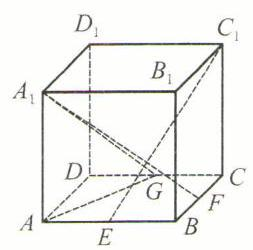
\includegraphics[width=0.2\textwidth]{bodyxb/src/bo_d20aucref24c73anc48g_230_1256_618_253_250_0.jpg}
\end{center}


(图 5)

(1)证明: ${C}_{1}E//$ 平面 ${A}_{1}{AG}$ ；

(2)证明: ${A}_{1}F \bot  {C}_{1}E$ .

分析 建立空间直角坐标系,求 ${C}_{1}E,{A}_{1}F$ 的方向向量和平面 ${A}_{1}{AG}$ 的法向量, 利用空间向量证明线面平行和线线垂直.

解 如图 6,以 $D$ 为坐标原点,分别以 $\vv{DA},\vv{DC}$ 与 ${\vv{DD}}_{1}$ 的方向为 $x$ , $y$ 与 $z$ 轴的正方向,建立空间直角坐标系,不妨设 ${AB} = 2$ ,则 $A\left( {2,0,0}\right)$ , ${A}_{1}\left( {2,0,2}\right) ,{C}_{1}\left( {0,2,2}\right) ,E\left( {2,1,0}\right) ,F\left( {1,2,0}\right) ,G\left( {0,1,0}\right)$ ,

\begin{center}
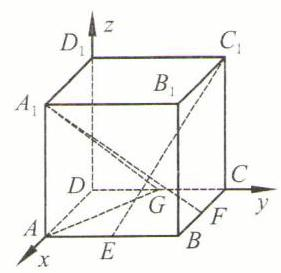
\includegraphics[width=0.2\textwidth]{bodyxb/src/bo_d20aucref24c73anc48g_230_1225_978_281_273_0.jpg}
\end{center}


(图 6)

可得 $\vv{{C}_{1}E} = \left( {2, - 1, - 2}\right) ,\vv{A{A}_{1}} = \left( {0,0,2}\right) ,\vv{AG} = \left( {-2,1,0}\right)$ ,

设平面 ${A}_{1}{AG}$ 的法向量为 $\vv{n} = \left( {x,y,z}\right)$ ,则 $\left\{  \begin{array}{l} \vv{n} \cdot  \vv{A{A}_{1}} = {2z} = 0, \\  \vv{n} \cdot  \vv{AG} =  - {2x} + y = 0, \end{array}\right.$

令 $x = 1$ ,则 $y = 2,z = 0$ ,可得 $\vv{n} = \left( {1,2,0}\right)$ ,

因为 $n \cdot  \vv{{C}_{1}E} = 2 - 2 = 0$ ,且 $E{C}_{1}$ 在平面 ${A}_{1}{AG}$ 外,所以 ${C}_{1}E//$ 平面 ${A}_{1}{AG}$ .

(2) 由 (1) 可得 $\vv{{A}_{1}F} = \left( {-1,2, - 2}\right)$ ,则 $\vv{{A}_{1}F} \cdot  \vv{{C}_{1}E} =  - 2 - 2 + 4 = 0$ ,所以 ${A}_{1}F \bot  {C}_{1}E$ .

例 4 如图 7,在四棱锥 $P - {ABCD}$ 中,底面 ${ABCD}$ 是矩形, ${PA} \bot$ 底面 ${ABCD},{PA} = {AB} = 2,{AD} = 1,E$ 是 ${PB}$ 的中点,点 $F$ 在棱 ${BC}$ 上,且 $\vv{PF} = \dfrac{4}{9}\vv{PC}$ .

\begin{center}
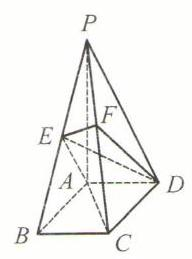
\includegraphics[width=0.2\textwidth]{bodyxb/src/bo_d20aucref24c73anc48g_230_1319_1517_192_259_0.jpg}
\end{center}


(图 7)

求证: ${PC} \bot$ 平面 ${AEF}$ .

分析 建立空间直角坐标系,分别求得 $\vv{PC},\vv{AE}$ 和 $\vv{AF}$ 的坐标,通过计算证明 $\vv{PC} \bot  \vv{AE}$ 及 $\vv{PC} \bot  \vv{AF}$ ,从而说明 ${PC} \bot$ 平面 ${AEF}$ .

证明 如图 8,以 $A$ 为原点,分别 $\vv{AB},\vv{AD}$ 和 $\vv{AP}$ 的方向为 $x\text{ 、 }y$ 与 $z$ 轴的正方向,建立空间直角坐标系,则 $P\left( {0,0,2}\right) ,C\left( {2,1,0}\right) ,E\left( {1,0,1}\right)$ ,

\begin{center}
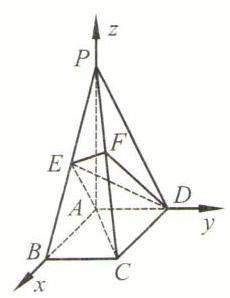
\includegraphics[width=0.2\textwidth]{bodyxb/src/bo_d20aucref24c73anc48g_230_1279_1844_230_298_0.jpg}
\end{center}


(图 8)

所以 $\vv{PC} = \left( {2,1, - 2}\right) ,\vv{AE} = \left( {1,0,1}\right)$ ,

$\vv{AF} = \vv{AP} + \vv{PF} = \vv{AP} + \dfrac{4}{9}\vv{PC} = \left( {\dfrac{8}{9},\dfrac{4}{9},\dfrac{10}{9}}\right) .$

因为 $\vv{PC} \cdot  \vv{AE} = 2 - 2 = 0$ ,且 $\vv{PC} \cdot  \vv{AF} = \dfrac{16}{9} + \dfrac{4}{9} - \dfrac{20}{9} = 0$ ,所以 $\vv{PC}\bot \vv{AE}$ 且 $\vv{PC}\bot \vv{AF}$ .

又因为 ${AE},{AF}$ 是平面 ${AEF}$ 内两相交直线,所以 ${PC} \bot$ 平面 ${AEF}$ .

例 5 如图 9,在四棱锥 $P - {ABCD}$ 中,底面 ${ABCD}$ 是正方形, ${PD} \bot$ 平面 ${ABCD},{PD} = {AD} = 2$ ,且 $E,F$ 分别为 ${AB}$ 和 ${PD}$ 中点.

\begin{center}
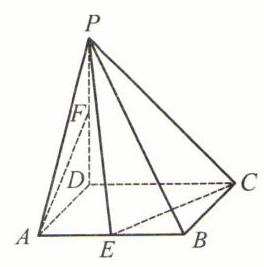
\includegraphics[width=0.2\textwidth]{bodyxb/src/bo_d20aucref24c73anc48g_231_1155_284_264_267_0.jpg}
\end{center}


(图 9)

(1)求异面直线 ${AF}$ 与 ${EC}$ 所成角的余弦值；

(2)求点 $F$ 到直线 ${EC}$ 的距离.

分析 建立空间直角坐标系,分别求得向量 $\vv{AF},\vv{EC}$ 的坐标,异面直线 ${AF}$ 与 ${EC}$ 的所成角 $\theta$ 由公式 $\cos \theta  = \dfrac{\left| \vv{AF} \cdot  \vv{EC}\right| }{\left| \vv{AF}\right| \left| \vv{EC}\right| }$ 确定;

先求 $\vv{CF}$ 在 $\vv{CE}$ 方向上的投影向量的模 $m$ ,再利用勾股定理求点 $F$ 到直线 ${EC}$ 的距离 $d$  $= \sqrt{{\left| \vv{CF}\right| }^{2} - {m}^{2}}$ .

解 以 $D$ 为坐标原点,分别以 $\vv{DA},\vv{DC}$ 与 $\vv{DP}$ 的方向为 $x,y$ 与 $z$ 轴的正方向,建立空间直角坐标系,得 $A\left( {2,0,0}\right) ,P\left( {0,0,2}\right) ,F\left( {0,0,1}\right) ,E\left( {2,1,0}\right) ,C\left( {0,2,0}\right)$ .

(1) $\vv{AF} = \left( {-2,0,1}\right) ,\vv{EC} = \left( {-2,1,0}\right)$ ,设异面直线 ${AF}$ 与 ${EC}$ 的所成角为 $\theta$ ,

则 $\cos \theta  = \dfrac{\left| \vv{AF} \cdot  \vv{EC}\right| }{\left| \vv{AF}\right| \left| \vv{EC}\right| } = \dfrac{4}{5}$ ,故异面直线 ${AF}$ 与 ${EC}$ 所成角的余弦值为 $\dfrac{4}{5}$ .

(2) $\vv{CF} = \left( {0, - 2,1}\right) ,\vv{CE} = \left( {2, - 1,0}\right) ,\vv{CF}$ 在 $\vv{CE}$ 方向上的投影向量的模 $m = \dfrac{\left| \vv{CF} \cdot  \vv{CE}\right| }{\left| \vv{EC}\right| }$  $= \dfrac{2}{\sqrt{5}}$ ,故点 $F$ 到直线 ${EC}$ 的距离 $d = \sqrt{{\left| \vv{CF}\right| }^{2} - {m}^{2}} = \sqrt{5 - \dfrac{4}{5}} = \dfrac{\sqrt{105}}{5}$ .

\begin{center}
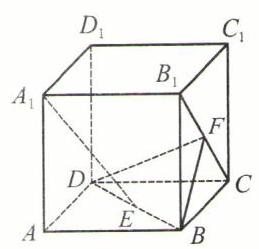
\includegraphics[width=0.2\textwidth]{bodyxb/src/bo_d20aucref24c73anc48g_231_1166_1241_259_249_0.jpg}
\end{center}


(图 10)

例 6 如图 10,在正方体 ${ABCD} - {A}_{1}{B}_{1}{C}_{1}{D}_{1}$ 中, ${AB} = 2,E,F$ 分别是 ${BD},{B}_{1}C$ 的中点.

(1)求直线 ${A}_{1}E$ 与平面 ${BDF}$ 所成角的正弦值；

(2)求点 ${A}_{1}$ 到平面 ${BDF}$ 的距离.

分析 根据题意建立空间直角坐标系,求出平面 ${BDF}$ 的法向量和向量 $\vv{{A}_{1}E}$ 的坐标,然后分别利用线面所成角正弦值的计算公式和点到平面的距离公式即可求解.

解 如图 11,以 $D$ 为坐标原点,分别以 $\vv{DA},\vv{DC}$ 与 ${\vv{DD}}_{1}$ 的方向为 $x,y$ 与 $z$ 轴的正方向,建立空间直角坐标系,则 $B\left( {2,2,0}\right) ,{A}_{1}\left( {2,0,2}\right) ,E$  $\left( {1,1,0}\right) ,F\left( {1,2,1}\right)$ ,

\begin{center}
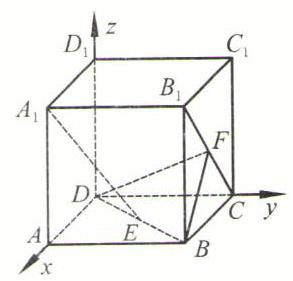
\includegraphics[width=0.2\textwidth]{bodyxb/src/bo_d20aucref24c73anc48g_231_1135_1644_293_281_0.jpg}
\end{center}


(图 11)

则 $\vv{DB} = \left( {2,2,0}\right) ,\vv{DF} = \left( {1,2,1}\right) ,\vv{{A}_{1}E} = \left( {-1,1, - 2}\right)$ .

设平面 ${BDF}$ 的法向量 $\vv{n} = \left( {x,y,z}\right)$ ,则 $\left\{  \begin{array}{l} \vv{n} \cdot  \vv{DB} = {2x} + {2y} = 0, \\  \vv{n} \cdot  \vv{DF} = x + {2y} + z = 0, \end{array}\right.$

令 $y =  - 1$ ,得平面 ${BDF}$ 的一个法向量 $\vv{n} = \left( {1, - 1,1}\right)$ .

(1)设直线 ${A}_{1}E$ 与平面 ${BDF}$ 所成角为 $\theta$ ,则 $\sin \theta  = \dfrac{\left| \vv{{A}_{1}E} \cdot  \vv{n}\right| }{\left| \vv{{A}_{1}E}\right| \left| \vv{n}\right| } = \dfrac{4}{\sqrt{6} \cdot  \sqrt{3}} = \dfrac{2\sqrt{2}}{3}$ .

(2)点 ${A}_{1}$ 到平面 ${BDF}$ 的距离 $d = \dfrac{\left| \vv{{A}_{1}E} \cdot  \vv{n}\right| }{\left| \vv{n}\right| } = \dfrac{4}{\sqrt{3}} = \dfrac{4\sqrt{3}}{3}$ .

例 7 如图 12,在三棱锥 $A - {BCD}$ 中,平面 ${ABD} \bot$ 平面 ${BCD},{AB} =$  ${AD},O$ 为 ${BD}$ 的中点, $\bigtriangleup {OCD}$ 是边长为 1 的等边三角形,且 ${V}_{A - {BCD}} = \dfrac{\sqrt{3}}{6}$ .

\begin{center}
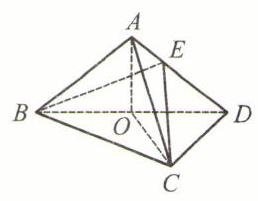
\includegraphics[width=0.2\textwidth]{bodyxb/src/bo_d20aucref24c73anc48g_232_1265_260_258_201_0.jpg}
\end{center}


(图 12)

(1)求直线 ${CD}$ 与平面 ${ABC}$ 所成角的正弦值；

(2)在棱 ${AD}$ 上是否存在点 $E$ ,使二面角 $E - {BC} - D$ 的大小为 ${45}^{ \circ  }$ ？若存在,求出 $\dfrac{AE}{DE}$ 的值; 若不存在,请说明理由.

分析 先求得 ${CD},{BC},{OA}$ 的长度,然后建立空间直角坐标系.

(1)利用向量法求得直线 ${CD}$ 和平面 ${ABC}$ 所成角的正弦值；(2)设 $\vv{AE} = \lambda \vv{AD}$  $\left( {0 \leq  \lambda  \leq  1}\right)$ ,利用二面角 $E - {BC} - D$ 的大小列方程,求得 $\lambda$ ,进而求得 $\dfrac{AE}{DE}$ .

解 由题意知, ${AO} \bot  {BD}$ ,又平面 ${ABD} \bot$ 平面 ${BCD}$ ,平面 ${ABD} \cap$ 平面 ${BCD} = {BD},{AO} \subset$ 平面 ${ABD}$ ,所以 ${AO} \bot$ 平面 ${BCD}$ . 因为 ${V}_{A - {BCD}} = \dfrac{1}{3}{S}_{\bigtriangleup {BCD}}$  $\cdot  {AO} = \dfrac{1}{3} \cdot  \dfrac{\sqrt{3}}{2} \cdot  {AO} = \dfrac{\sqrt{3}}{6}$ ,所以 ${AO} = 1$ . 分别取 ${BC},{CD}$ 的中点 $F,G$ ,易证 ${OA},{OF}$ 与 ${OG}$ 两两垂直. 如图 13,以 $O$ 为坐标原点,分别以 $\vv{OF},\vv{OG}$ 与 $\vv{OA}$ 的方向为 $x,y$ 与 $z$ 轴的正方向,建立空间直角坐标系,则 $A\left( {0,0,1}\right) ,B\left( {\dfrac{1}{2}, - \dfrac{\sqrt{3}}{2},0}\right)$ ,

\begin{center}
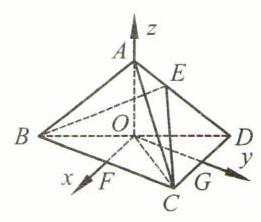
\includegraphics[width=0.2\textwidth]{bodyxb/src/bo_d20aucref24c73anc48g_232_1262_846_261_222_0.jpg}
\end{center}


(图 13)

$C\left( {\dfrac{1}{2},\dfrac{\sqrt{3}}{2},0}\right) ,D\left( {-\dfrac{1}{2},\dfrac{\sqrt{3}}{2},0}\right) ,F\left( {\dfrac{1}{2},0,0}\right) ,G\left( {0,\dfrac{\sqrt{3}}{2},0}\right)$ .

(1) $\vv{AB} = \left( {\dfrac{1}{2}, - \dfrac{\sqrt{3}}{2}, - 1}\right) ,\vv{BC} = \left( {0,\sqrt{3},0}\right) ,\vv{CD} = \left( {-1,0,0}\right)$ ,

设平面 ${ABC}$ 的法向量 ${\vv{n}}_{1} = \left( {{x}_{1},{y}_{1},{z}_{1}}\right)$ ,则 $\left\{  \begin{array}{l} \vv{n} \cdot  \vv{AB} = \dfrac{1}{2}{x}_{1} - \dfrac{\sqrt{3}}{2}{y}_{1} - {z}_{1} = 0 \\  \vv{n} \cdot  \vv{BC} = \sqrt{3}{y}_{1} = 0, \end{array}\right.$

令 ${x}_{1} = 2$ ,得平面 ${ABC}$ 的一个法向量 $\vv{n} = \left( {2,0,1}\right)$ .

设直线 ${CD}$ 与平面 ${ABC}$ 的所成角为 $\theta$ ,则 $\sin \theta  = \dfrac{\left| \vv{CD} \cdot  \vv{n}\right| }{\left| \vv{CD}\right| \left| \vv{n}\right| } = \dfrac{2}{\sqrt{5}} = \dfrac{2\sqrt{5}}{5}$ .

(2)设 $\vv{AE} = \lambda \vv{AD} = \left( {-\dfrac{1}{2}\lambda ,\dfrac{\sqrt{3}}{2}\lambda , - \lambda }\right) ,0 \leq  \lambda  \leq  1$ ,

$\vv{BE} = \vv{AE} - \vv{AB} = \left( {-\dfrac{\lambda  + 1}{2},\dfrac{\sqrt{3}\left( {\lambda  + 1}\right) }{2}, - \lambda  + 1}\right) ,\vv{OA} = \left( {0,0,1}\right)$ 是平面 ${BCD}$ 的一个法向量,

设 ${\vv{n}}_{2} = \left( {{x}_{2},{y}_{2},{z}_{2}}\right)$ 是平面 ${BCE}$ 的一个法向量,则

$\left\{  \begin{array}{l} {\vv{n}}_{2} \cdot  \vv{BC} = \sqrt{3}{y}_{2} = 0, \\  {\vv{n}}_{2} \cdot  \vv{BE} =  - \dfrac{\lambda  + 1}{2}{x}_{2} + \dfrac{\sqrt{3}\left( {\lambda  + 1}\right) }{2}{y}_{2} + \left( {-\lambda  + 1}\right) {z}_{2} = 0. \end{array}\right.$ 可取 ${\vv{n}}_{2} = \left( {{2\lambda } - 2,0, - \lambda  - 1}\right)$ ,

因为二面角 $E - {BC} - D$ 的大小为 ${45}^{ \circ  }$ ,所以

$\left| {\cos \left\langle  {{\vv{n}}_{2},\vv{OA}}\right\rangle  }\right|  = \dfrac{\left| {\vv{n}}_{2} \cdot  \vv{OA}\right| }{\left| {\vv{n}}_{2}\right| \left| \vv{OA}\right| } = \dfrac{\left| \lambda  + 1\right| }{\sqrt{{\left( 2\lambda  - 2\right) }^{2} + {\left( \lambda  + 1\right) }^{2}}} = \dfrac{\sqrt{2}}{2}$ ,解得 $\lambda  = \dfrac{1}{3}$ .

故在棱 ${AD}$ 上存在点 $E$ ,使二面角 $E - {BC} - D$ 的大小为 ${45}^{ \circ  }$ ,此时, $\dfrac{AE}{DE} = \dfrac{1}{2}$ .

\section*{【训练题】}

\section*{(A)}

31. 空间直角坐标系中,点 $P\left( {1,2,3}\right)$ 关于平面 ${xOy}$ 的对称点是 (   )

(A)(-1, - 2,3). (B)(-1,2,3) (C)(1, - 2,3) (D)(1,2, - 3)

32. 已知向量 $\vv{a} = \left( {-3,2,5}\right) ,\vv{b} = \left( {1,5, - 1}\right)$ ,则 $\vv{a} - 2\vv{b} =$ (   )

(A)(-4, - 3,4). (B)(-5, - 8,7).

(C)(-5, - 8,3). (D)(-1, - 3,6).

33. 已知 $\vv{a} = \left( {2,2,1}\right) ,\vv{b} = \left( {1,1,0}\right)$ ,则 $\vv{a}$ 在 $\vv{b}$ 上的投影向量的坐标为(   )

(A)(1,1,0). (B)(1,2,0). (C)(2,2,0). (D)(1,1,1).

34. 已知向量 $\vv{a} = \left( {1,1,0}\right) ,\vv{b} = \left( {-1,0, - 2}\right)$ ,且 $k\vv{a} + \vv{b}$ 与 $2\vv{a} - \vv{b}$ 互相垂直,则 $k$ 的值是(   )

(A) 1 . (B) $\dfrac{1}{5}$ . (C) $\dfrac{3}{5}$ . (D) $\dfrac{7}{5}$ .

35. 设 $x,y \in  \mathbf{R},a = \left( {1,1,1}\right) ,b = \left( {1,y,z}\right) ,c = \left( {x, - 4,2}\right)$ ,且 $a \bot  c,b//c$ ,则 $\left| {{2a} + b}\right|  =$ (   )

(A) $2\sqrt{2}$ . (B) 0 . (C) 3 . (D) $3\sqrt{2}$ .

36. 已知 $\vv{a} = \left( {3, - 1,2}\right) ,\vv{b} = \left( {4,3, - 2}\right) ,\vv{c} = \left( {1,4,\lambda }\right)$ ,若 $\vv{a},\vv{b},\vv{c}$ 共面,则实数 $\lambda$ 的值为(   )

(A) -4. (B) -2 . (C) 2. (D) 4 .

37. 已知向量 $\vv{a} = \left( {2,4,x}\right) ,\vv{b} = \left( {2,y,2}\right)$ ,若 $\left| \vv{a}\right|  = 6,\vv{a}\bot \vv{b}$ ,则 $x + y$ 的值是 (   )

(A) -3 或 1 . (B) 3 或 -1 . (C)-3. (D) 1 .

38. 已知 $\vv{a} = \left( {1, - 2, - 1}\right) ,\vv{b} = \left( {-1,x - 1,1}\right)$ ,且 $\vv{a}$ 与 $\vv{b}$ 夹角为钝角,则 $x$ 的取值范围是(   )

(A) $\left( {0, + \infty }\right)$ . (B)(0,3).

(C) $\left( {3, + \infty }\right)$ . (D) $\left( {0,3}\right)  \cup  \left( {3, + \infty }\right)$ .

39. 已知平面 $\alpha$ 上的两个向量 $\vv{a} = \left( {2,3,1}\right) ,\vv{b} = \left( {5,6,4}\right)$ ,则平面 $\alpha$ 的一个法向量为 (   )

(A)(1, - 1,1). (B)(2, - 1,1). (C)(-2,1,1). (D)(-1,1,1).

40. 已知直线 $l$ 的一个方向向量为 $\mathbf{u} = \left( {1,0,1}\right)$ ,平面 $\alpha$ 的一个法向量为 $\vv{n} = \left( {0, - 1,1}\right)$ ,则 $l$ 与 $\alpha$ 所成角的正弦值为 (   )

(A) $\dfrac{1}{2}$ . (B) $\dfrac{\sqrt{3}}{2}$ . (C) $\dfrac{\sqrt{2}}{2}$ . (D) 1 .

41. 已知点 $O\left( {0,0,0}\right) ,A\left( {1,0,1}\right) ,B\left( {-1,1,2}\right) ,C\left( {-1,0, - 1}\right)$ ,则异面直线 ${OC}$ 与 ${AB}$ 所成角的正弦值为(   )

(A) $\dfrac{\sqrt{3}}{6}$ . (B) $\dfrac{\sqrt{3}}{3}$ . (C) $\dfrac{\sqrt{2}}{4}$ . (D) $\dfrac{\sqrt{33}}{6}$ .

42. 正方体 ${ABCD} - {A}_{1}{B}_{1}{C}_{1}{D}_{1}$ 中, $E$ 为 ${AB}$ 中点,则异面直线 ${A}_{1}E,{C}_{1}D$ 所成角的余弦值为(   )

(A) $\dfrac{\sqrt{15}}{15}$ . (B) $\dfrac{\sqrt{10}}{10}$ . (C) $\dfrac{1}{2}$ . (D) $\dfrac{\sqrt{3}}{3}$ .

43. 在正方体 ${ABCD} - {A}_{1}{B}_{1}{C}_{1}{D}_{1}$ 中, $E$ 为 ${BC}$ 的中点,则直线 ${D}_{1}E$ 与平面 ${AC}{D}_{1}$ 所成角的正弦值为(   )

(A) $\dfrac{1}{3}$ . (B) $\dfrac{\sqrt{3}}{9}$ . (C) $\dfrac{\sqrt{2}}{9}$ . (D) $\dfrac{1}{9}$ .

44. 四棱锥 $S - {ABCD}$ 中, $\vv{AB} = \left( {4, - 2,3}\right) ,\vv{AD} = \left( {-4,1,0}\right) ,\vv{AS} = \left( {-3,1, - 4}\right)$ ,则顶点 $S$ 到底面 ${ABCD}$ 的距离为(   )

(A) 1 . (B) 2 . (C) 3. (D) 4 .

45. 在空间直角坐标系中,已知 $A\left( {1,1, - 1}\right) ,B\left( {1,2,2}\right) ,C\left( {-3,4,2}\right)$ ,则点 $A$ 到直线 ${BC}$ 的距离为(   )

(A) $\dfrac{7\sqrt{5}}{5}$ . (B) $\sqrt{10}$ . (C) $\dfrac{\sqrt{39}}{2}$ . (D) $\dfrac{3\sqrt{5}}{2}$ .

46. 已知 $\vv{a} = \left( {1, - 2,3}\right) ,\vv{b} = \left( {2,m,n}\right)$ ,若 $\vv{a}//\vv{b}$ ,则 $m + n =$ \blkda{}.

47. 已知向量 $\vv{a} = \left( {2,\lambda , - 1}\right) ,\vv{b} = \left( {2,1, - 4}\right)$ ,若 $\vv{a}\bot \vv{b}$ ,则 $\lambda  =$ \blkda{}.

48. 已知向量 $\vv{a} = \left( {\sqrt{3},0,1}\right) ,\vv{b} = \left( {k,2,0}\right)$ ,若 $\vv{a}$ 与 $\vv{b}$ 的夹角为 $\dfrac{\pi }{3}$ ,则 $k$ 的值为\blkda{}.

49. 空间向量 $\vv{a} = \left( {2,2, - 1}\right)$ 的单位向量的坐标是\blkda{}.

50. 已知平面 $\alpha$ 的法向量为 $n = \left( {-1,2,1}\right) ,\vv{AB} = \left( {3,x,1}\right)$ ,若直线 ${AB}$ 与平面 $\alpha$ 平行,则 $x =$ \blkda{}.

51. 在空间直角坐标系中,点 $A\left( {2, - 1,3}\right)$ 关于平面 ${xOz}$ 的对称点为 $B$ ,则 $\vv{OA} \cdot  \vv{OB}$  $=$ \blkda{}.

52. 已知 $\left| \vv{a}\right|  = 3,\vv{b} = \left( {1,2, - 2}\right) ,\vv{a} \cdot  \vv{b} = 2$ ,则 $\left| {2\vv{a} - \vv{b}}\right|  =$ \blkda{}.

53. 已知向量 $\vv{a} = \left( {0,2,0}\right) ,\vv{b} = \left( {1, - 1,0}\right)$ ,则 $\vv{a}$ 在 $\vv{b}$ 方向上的投影向量的坐标为\blkda{}.

54. 已知空间两点 $A\left( {1,2, - 1}\right) ,B\left( {2,0,1}\right)$ ,点 $P\left( {-1,a,b}\right)$ 在直线 ${AB}$ 上运动,则 ${ab} =$ \blkda{}.

55. 已知点 $A\left( {0,0,1}\right) ,B\left( {0,1,0}\right) ,C\left( {1,0,0}\right)$ . 若点 $P\left( {x,1,2}\right)$ 在平面 ${ABC}$ 内,则 $x =$ \blkda{}.

\begin{center}
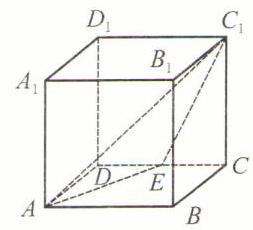
\includegraphics[width=0.2\textwidth]{bodyxb/src/bo_d20aucref24c73anc48g_234_1265_1858_253_230_0.jpg}
\end{center}


(第 56 题)

56. 如图,已知正方体 ${ABCD} - {A}_{1}{B}_{1}{C}_{1}{D}_{1}$ 的棱长为 $1,E$ 为棱 ${CD}$ 的中点, 则点 ${A}_{1}$ 到平面 ${AE}{C}_{1}$ 的距离为\blkda{}.

57. 已知 ${AB}$ 是圆锥 ${PO}$ 的底面直径, $C$ 是底面圆周上的一点, ${PC} = {AB} = 2,{AC} = \sqrt{3}$ ,则二面角 $A - {PB} - C$ 的余弦值为\blkda{}.

58. 如图,在三棱柱 ${ABC} - {A}_{1}{B}_{1}{C}_{1}$ 中, ${AB}$ , ${AC}$ , $A{A}_{1}$ 两两垂直, ${AB} = 1$ , ${AC} = \sqrt{2}$ , $A{A}_{1} = 2$ , $D$ 为 $C{C}_{1}$ 的中点,以 $A$ 为原点, $\vv{AB},\vv{AC}$ 与 $\vv{A{A}_{1}}$ 的方向为 $x,y$ 与 $z$ 轴的正方向,建立空间直角坐标系.

(1)求证: ${A}_{1}C\bot {BD}$ ；

(2)求直线 ${A}_{1}C$ 与平面 $A{B}_{1}C$ 所成角的正弦值；

(3)求点 ${A}_{1}$ 到平面 $A{B}_{1}C$ 的距离.

\begin{center}
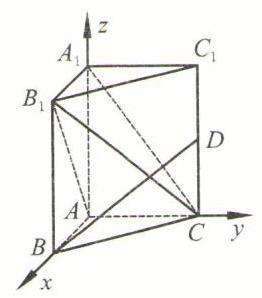
\includegraphics[width=0.2\textwidth]{bodyxb/src/bo_d20aucref24c73anc48g_235_239_633_262_298_0.jpg}
\end{center}


(第 58 题)

\begin{center}
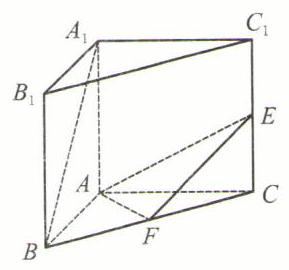
\includegraphics[width=0.2\textwidth]{bodyxb/src/bo_d20aucref24c73anc48g_235_612_660_289_270_0.jpg}
\end{center}


(第 59 题)

\begin{center}
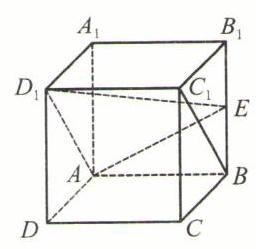
\includegraphics[width=0.2\textwidth]{bodyxb/src/bo_d20aucref24c73anc48g_235_1009_677_256_249_0.jpg}
\end{center}


(第 60 题)

59. 如图,在直三棱柱 ${ABC} - {A}_{1}{B}_{1}{C}_{1}$ 中, ${AB} = {AC} = {A{A}_{1}} = 2,\angle {BAC} = {90}^{ \circ  },E,F$ 分别为 $C{C}_{1},{BC}$ 的中点.

(1)求直线 ${A}_{1}B$ 与直线 ${EF}$ 所成角的大小；

(2)求平面 ${AB}{A}_{1}$ 与平面 ${AEF}$ 所成的锐二面角的大小.

60. 如图,在正方体 ${ABCD} - {A}_{1}{B}_{1}{C}_{1}{D}_{1}$ 中, $E$ 为 $B{B}_{1}$ 的中点.

(1)求证: $B{C}_{1}//$ 平面 $A{D}_{1}E$ ；

(2)求直线 $A{A}_{1}$ 与平面 $A{D}_{1}E$ 所成角的正弦值.

61. 如图,在长方体 ${ABCD} - {A}_{1}{B}_{1}{C}_{1}{D}_{1}$ 中, ${AD} = 1$ , ${AB} = {A{A}_{1}} = 2$ , $H$ , $F$ 分别是棱 ${C}_{1}{D}_{1}$ , $B{B}_{1}$ 的中点.

(1)求直线 ${HF}$ 与平面 ${ABCD}$ 所成角的大小；

(2)在线段 ${HF}$ 上是否存在一点 $Q$ ,使得 $Q$ 到平面 ${A}_{1}{BC}{D}_{1}$ 的距离是 $\sqrt{2}$ . 若存在,求出 $\dfrac{HQ}{HF}$ 的值; 若不存在,说明理由.

\begin{center}
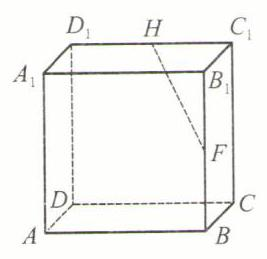
\includegraphics[width=0.2\textwidth]{bodyxb/src/bo_d20aucref24c73anc48g_235_452_1748_267_259_0.jpg}
\end{center}


(第 61 题)

\begin{center}
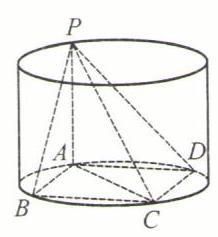
\includegraphics[width=0.2\textwidth]{bodyxb/src/bo_d20aucref24c73anc48g_235_860_1759_218_237_0.jpg}
\end{center}


(第 62 题)

62. 如图,四棱锥 $P - {ABCD}$ 的底面 ${ABCD}$ 是圆柱底面圆的内接矩形, ${PA}$ 是圆柱的母线, ${PA}$  $= {AD} = 2,{AB} = 1$ .

(1)证明:平面 ${PCD} \bot$ 平面 ${PAD}$ ；

(2)求平面 ${PBC}$ 与平面 ${PCD}$ 所成的锐二面角的余弦值.

\section*{(B)}

63. 设 ${A}_{1},{A}_{2},\cdots ,{A}_{n}$ 是空间中给定的 $n$ 个不同的点,则使 $\mathop{\sum }\limits_{{i = 1}}^{n}\left( {i\vv{M{A}_{i}}}\right)  = \vv{0}$ 成立的点 $M$ 的个数为(   )

(A) 1 . (B) $n$ .

(C) 无穷多个. (D) 以上说法都有可能.

64. 空间直角坐标系 $O - {xyz}$ 中,经过点 $P\left( {{x}_{0},{y}_{0},{z}_{0}}\right)$ 且法向量为 $m = \left( {A,B,C}\right)$ 的平面方程为 $A\left( {x - {x}_{0}}\right)  + B\left( {y - {y}_{0}}\right)  + C\left( {z - {z}_{0}}\right)  = 0$ ,经过点 $\left( {{x}_{0},{y}_{0},{z}_{0}}\right)$ 且一个方向向量为 $\vv{n} = (a$ , $b,c)\left( {{abc} \neq  0}\right)$ 的直线 $l$ 的方程为 $\dfrac{x - {x}_{0}}{a} = \dfrac{y - {y}_{0}}{b} = \dfrac{z - {z}_{0}}{c}$ ,阅读上面的材料并解决下列问题: 现给出平面 $\alpha$ 的方程为 ${2x} - {3y} - z = 0$ ,经过点(0,0,0)的直线 $l$ 的方程为 $\dfrac{x}{-1} = \dfrac{y}{2} =$  $\dfrac{z}{-3}$ ,则直线 $l$ 与平面 $\alpha$ 所成角的正弦值为 (   )

(A) $\dfrac{5}{14}$ . (B) $\dfrac{3}{14}$ . (C) $\dfrac{5}{13}$ . (D) $\dfrac{3}{13}$ .

65. 钟鼓楼是中国传统建筑之一,属于钟楼和鼓楼的合称,是主要用于报时的建筑. 中国古代一般建于城市的中心地带, 在现代城市中, 也可以常常看见附有钟楼的建筑. 如图, 在某市一建筑物楼顶有一顶部逐级收拢的四面钟楼,四个大钟对称分布在四棱柱的四个侧面 (四棱柱看成正四棱柱,钟面圆心在棱柱侧面中心上), 在整点时刻 (在 0 点至 12 点中取整数点,含 0 点,不含 12 点),已知在 3 点时和 9 点时,相邻两钟面上的时针所在的两条直线相互垂直, 则在 2 点时和 8 点时, 相邻两钟面上的时针所在的两条直线所成的角的余弦值为(   )

\begin{center}
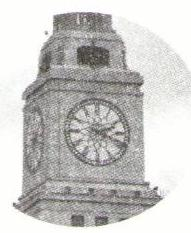
\includegraphics[width=0.2\textwidth]{bodyxb/src/bo_d20aucref24c73anc48g_236_1307_1131_191_233_0.jpg}
\end{center}


(第 65 题)

(A) $\dfrac{\sqrt{2}}{6}$ . (B) $\dfrac{1}{4}$ . (C) $\dfrac{\sqrt{3}}{6}$ . (D) $\dfrac{\sqrt{2}}{4}$ .

66. 如图,已知正方体 ${ABCD} - {A}_{1}{B}_{1}{C}_{1}{D}_{1}$ 的棱长为 $1,M$ 为棱 ${AB}$ 的中点, 点 $P$ 在正方形 ${BC}{C}_{1}{B}_{1}$ 内部 (不含边界) 运动,给出以下三个结论:

\begin{center}
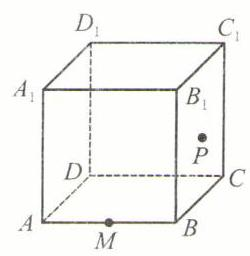
\includegraphics[width=0.2\textwidth]{bodyxb/src/bo_d20aucref24c73anc48g_236_1259_1690_250_256_0.jpg}
\end{center}


(第 66 题)

① 存在点 $P$ 满足 $P{D}_{1} \bot  M{B}_{1}$ ；

②存在点 $P$ 满足 $P{D}_{1}$ 与平面 ${A}_{1}{D}_{1}M$ 所成角的大小为 ${60}^{ \circ  }$ ；

③ 存在点 $P$ 满足 $M{D}_{1} + {MP} = \dfrac{12}{5}$ .

其中正确的个数是 (   ).

(A) 0 . (B) 1 . (C) 2 . (D) 3.

67. 在正方体 ${ABCD} - {A}_{1}{B}_{1}{C}_{1}{D}_{1}$ 中, $E$ 为棱 $B{B}_{1}$ 的中点, $P$ 是正方体内 (含边界)一点,满足 ${C}_{1}P \bot  {A}_{1}E$ . 若 ${AB} = 2$ ,则 $\vv{P{A}_{1}} \cdot  \vv{P{D}_{1}}$ 的取值范围是\blkda{}.

\begin{center}
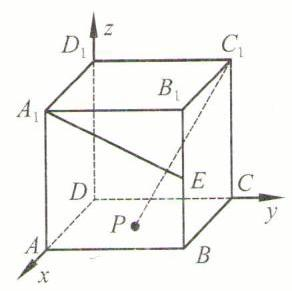
\includegraphics[width=0.2\textwidth]{bodyxb/src/bo_d20aucref24c73anc48g_237_400_255_292_291_0.jpg}
\end{center}


(第 67 题)

\begin{center}
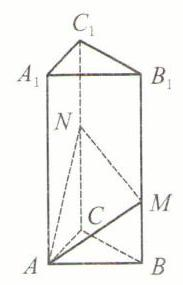
\includegraphics[width=0.2\textwidth]{bodyxb/src/bo_d20aucref24c73anc48g_237_876_257_183_285_0.jpg}
\end{center}


(第 69 题)

68. 在空间直角坐标系中,已知 $A\left( {0,3,2}\right) ,B\left( {0,\dfrac{3}{2},2}\right) ,C\left( {2,\dfrac{3}{2},2}\right) ,{A}_{1}\left( {0,3,0}\right) ,{B}_{1}\left( {0,0,0}\right)$ , ${C}_{1}\left( {4,0,0}\right)$ ,则几何体 ${ABC} - {A}_{1}{B}_{1}{C}_{1}$ 的体积为\blkda{}.

69. 如图,在三棱柱中 ${ABC} - {A}_{1}{B}_{1}{C}_{1}$ 中, ${AB}$ , ${AC}$ , $A{A}_{1}$ 两两互相垂直, $A{A}_{1} = {2AB} = {2AC}$ , $M,N$ 是线段 $B{B}_{1},C{C}_{1}$ 上的点,平面 ${AMN}$ 与平面 ${ABC}$ 所成锐二面角大小为 $\dfrac{\pi }{6}$ ,当 ${B}_{1}M$ 最小时, $\angle {AMB} =$ \blkda{}.

70. 直四棱柱 ${ABCD} - {A}_{1}{B}_{1}{C}_{1}{D}_{1}$ 的所有棱长都为 $2,\angle {BAD} = \dfrac{\pi }{3}$ ,点 $P$ 在四边形 ${BD}{D}_{1}{B}_{1}$ 及其内部运动,且满足 $\left| {PA}\right|  + \left| {PC}\right|  = 4$ ,则点 $P$ 到平面 $A{D}_{1}{B}_{1}$ 的距离的最小值为\blkda{}.

71. 如图,几何体是以正方形 ${ABCD}$ 的一边 ${BC}$ 所在直线为旋转轴,其余三边旋转 ${90}^{ \circ  }$ 形成的面所围成的几何体, $G$ 是圆弧 $\overset{⏜}{DF}$ 的中点, $H$ 是圆弧 $\overset{⏜}{AE}$ 上的动点, ${AB} = 2$ ,给出下列四个结论:

① 不存在点 $H$ ,使得平面 ${BDH}//$ 平面 ${CEG}$ ；

\begin{center}
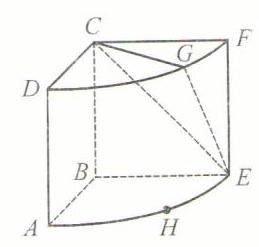
\includegraphics[width=0.2\textwidth]{bodyxb/src/bo_d20aucref24c73anc48g_237_1180_1355_259_247_0.jpg}
\end{center}


(第 71 题)

②存在点 $H$ ,使得 ${FH} \bot$ 平面 ${CEG}$ ；

③不存在点 $H$ ,使得点 $H$ 到平面 ${CEG}$ 的距离大于 $\dfrac{4\sqrt{3}}{3}$ ；

④ 存在点 $H$ ,使得直线 ${DH}$ 与平面 ${CEG}$ 所成角的正弦值为 $\dfrac{\sqrt{2}}{3}$ .

其中所有正确结论的序号是\blkda{}.

72. 如图,在四棱柱 ${ABCD} - {A}_{1}{B}_{1}{C}_{1}{D}_{1}$ 中,侧棱 ${A}_{1}A \bot$ 平面 ${ABCD}$ , ${AB}//{CD},{AB} \bot  {AD},{AD} = {CD} = 1,A{A}_{1} = {AB} = 2,E$ 为棱 $A{A}_{1}$ 的中点, $M$ 为线段 ${CE}$ 的中点.

\begin{center}
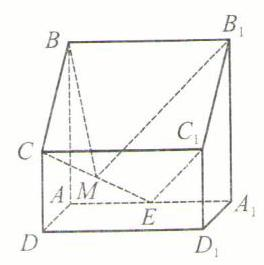
\includegraphics[width=0.2\textwidth]{bodyxb/src/bo_d20aucref24c73anc48g_237_1183_1738_264_265_0.jpg}
\end{center}


(第 72 题)

(1) 证明: ${BC} \bot  {C}_{1}E$ ;

(2)求异面直线 ${BM}$ 与 ${AD}$ 所成角的余弦值；

(3) 求点 ${C}_{1}$ 到平面 ${BM}{B}_{1}$ 的距离.

73. 如图,在四棱锥 $P - {ABCD}$ 中,底面 ${ABCD}$ 为菱形,且 ${AB} = 2,\angle {ABC}$  $= 2\angle {BAD},\angle {PDC} = \dfrac{\pi }{2},M$ 为棱 ${DP}$ 的中点.

\begin{center}
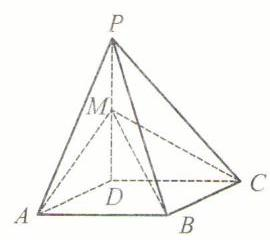
\includegraphics[width=0.2\textwidth]{bodyxb/src/bo_d20aucref24c73anc48g_238_1248_133_270_240_0.jpg}
\end{center}


(第 73 题)

(1)在棱 ${BC}$ 上是否存在一点 $N$ ,使得 ${CM}//$ 平面 ${PAN}$ ,并说明理由； (2)若 ${PB}\bot {AC}$ ,二面角 $B - {CM} - D$ 的余弦值为 $\dfrac{\sqrt{6}}{6}$ 时,求点 $A$ 到平面 ${BCM}$ 的距离.

74. 如图 1 是直角梯形 ${ABCD},{AB}//{CD},\angle D = {90}^{ \circ  },{AB} = 2,{CD} = 3,\angle {DCB} = {60}^{ \circ  },E$ 在线段 ${CD}$ 上,且 ${CE} = {2ED}$ ,以 ${BE}$ 为折痕将 $\bigtriangleup {BCE}$ 折起,使点 $C$ 到达 ${C}_{1}$ 的位置,且 $A{C}_{1} = \sqrt{6}$ , 如图 2.

(1)求证:平面 $B{C}_{1}E \bot$ 平面 ${ABED}$ ；

(2)在棱 $D{C}_{1}$ 上存在点 $P$ ,使得锐二面角 $P - {BE} - A$ 的大小为 ${45}^{ \circ  }$ ,求 ${C}_{1}$ 到平面 ${PBE}$ 的距离.

\begin{center}
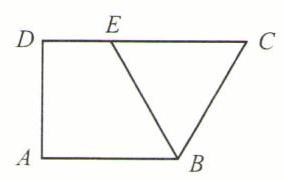
\includegraphics[width=0.2\textwidth]{bodyxb/src/bo_d20aucref24c73anc48g_238_559_880_284_181_0.jpg}
\end{center}


图 1

\begin{center}
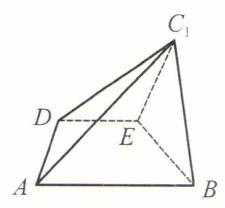
\includegraphics[width=0.2\textwidth]{bodyxb/src/bo_d20aucref24c73anc48g_238_888_856_225_208_0.jpg}
\end{center}


图 2

(第 74 题)

75. 如图,一个工作台的下半部分是个正四棱柱 ${ABCD} - {A}_{1}{B}_{1}{C}_{1}{D}_{1}$ ,其底面边长为 4,高为 1, 工作台的上半部分是一个底面半径 ${D}_{1}E$ 为 $\sqrt{2}$ ,母线 $E{E}_{1}$ 长为 3 的圆柱体的四分之一. 若 $P$ 是圆弧 ${E}_{1}{F}_{1}$ 上的动点,当平面 $P{A}_{1}{C}_{1}$ 与平面 ${ABC}$ 所成的钝二面角最大时,求点 $P$ 在圆弧上的位置.

\begin{center}
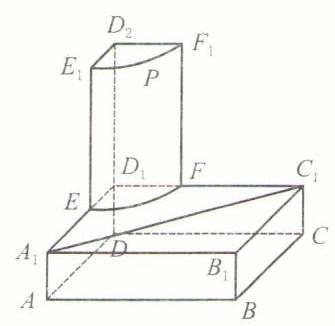
\includegraphics[width=0.2\textwidth]{bodyxb/src/bo_d20aucref24c73anc48g_238_1176_1445_335_326_0.jpg}
\end{center}


(第 75 题)
